
	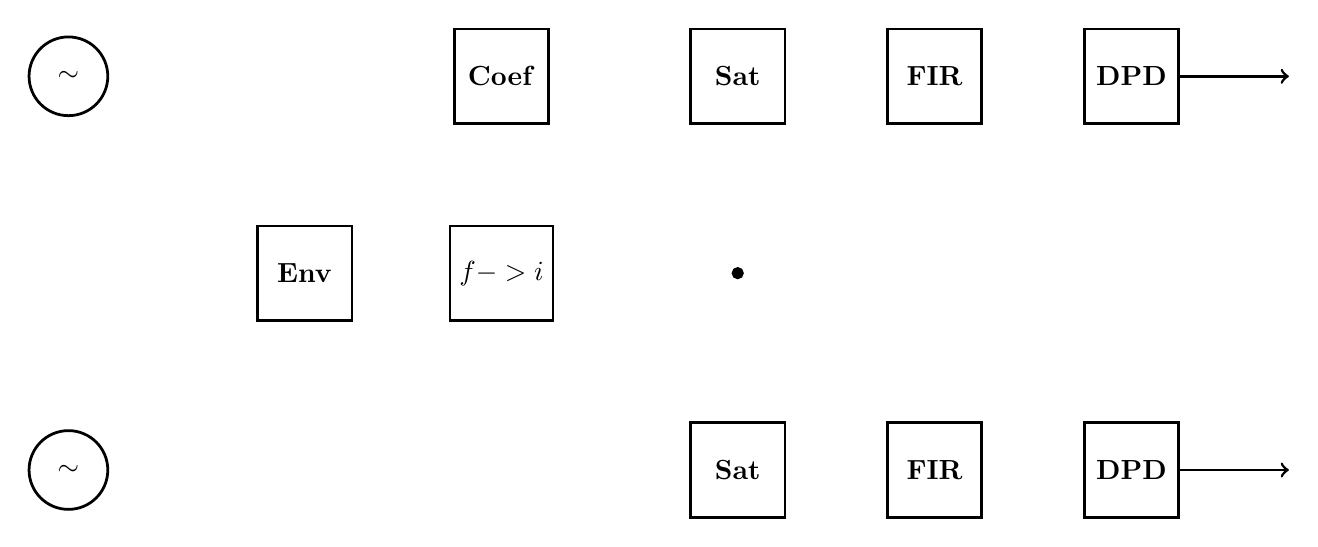
\begin{tikzpicture}[
		scale=1,
		transform shape,
		retangulos/.style={
			draw, 
			rectangle, 
			minimum width=1.2cm, 
			minimum height=1.2cm,
			align=center, 
			line width = 1pt
		},
		circulo/.style={
			draw,
			circle,
			minimum size=1cm,
			inner sep=0pt,      
			line width = 1pt,              
			align=center,       
			fill=white          
		}
		]
		
		\node[circulo] (S1) at (0,2.5) {$\sim$};
		\node[circulo] (S2) at (0,-2.5) {$\sim$};
		
		\node[retangulos] (Env) at (3,0) {\textbf{Env}};
		\node[retangulos] (int) at (5.5,0) {$f->i$};
		\node[retangulos] (Coef) at (5.5,2.5) {\textbf{Coef}};
		
		\filldraw [black] (8.5,0) circle (2pt);
		\node[retangulos] (sat1) at (8.5, 2.5) {\textbf{Sat}};
		\node[retangulos] (sat2) at (8.5, -2.5) {\textbf{Sat}};
		\node[retangulos] (fir1) at (11, 2.5) {\textbf{FIR}};
		\node[retangulos] (fir2) at (11, -2.5) {\textbf{FIR}};
		\node[retangulos] (dpd1) at (13.5, 2.5) {\textbf{DPD}};
		\node[retangulos] (dpd2) at (13.5, -2.5) {\textbf{DPD}};
		
		%Linhas
		\draw[->, line width=1pt] (dpd1.east) -- (15.5,2.5);
		\draw[->, line width=1pt] (dpd2.east) -- (15.5,-2.5) ;
		
	\end{tikzpicture}
